\section{Semantic Modeling of Computational Resources}
\label{sec:semantic}

In this work, we argue that in order to achieve reproducibility of a scientific workflow, enough information 
about the computational resources should be provided. These descriptions allow the target audience, 
usually another computational scientist in the same domain, to better understand the underlying 
components involved in a workflow execution.


% subsection
\subsection{WICUS ontology network}

We define semantic models for describing the main domains of a 
computational infrastructure, and for defining the taxonomy of concepts and the relationships 
between them. These models describe software components, hardware specifications, 
and computational resources (in the form of VMs). They also capture infrastructure 
dependencies of the workflows (e.g., services that must be running, available libraries, etc.).
 
 As a result, this process facilitates experiment's reusability since 
a new experiment, which may reuse parts of the workflow previously modeled, or a reproduction 
of a workflow, would benefit from the infrastructure dependencies already described.

We have identified four main domains of interest for documenting computational scientific 
infrastructures~\cite{wicus}, and developed a set of models, one for each domain, 
and an ontology network that defines the inter-domain relations between these models 
(Figure~\ref{fig:wicusrels}):

\begin{figure}[!t]
	\centering
	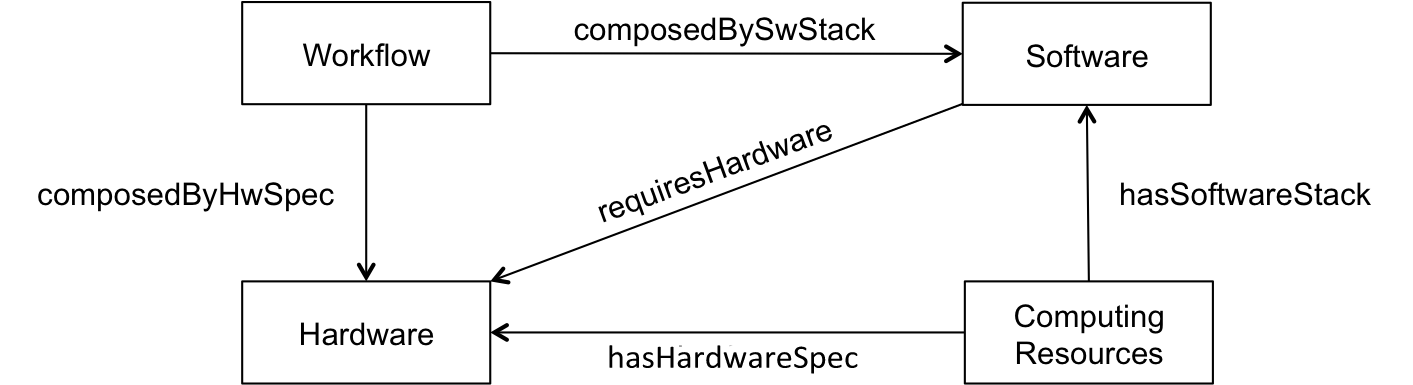
\includegraphics[width=.9\linewidth]{figures/wicusrels}
	\caption{Overview of the ontology network ($\rightarrow$ denotes inter-domain relation).}
	\label{fig:wicusrels}
\end{figure}

\begin{itemize}
	\setlength{\itemsep}{1pt}
	\setlength{\parskip}{0pt}
	\setlength{\parsep}{0pt}

	\item{\emph{Hardware domain}}: identifies the most common hardware information, 
		including CPU, Storage and RAM memory, and their capacities.
	
	\item{\emph{Software domain}}: defines the software components involved on the execution. 
    		It includes the pieces of executable software (e.g., scripts, binaries, and libraries) used in 
		the experiment. In addition, dependencies between those components and configuration 
		information are also defined, \rev{as well as the steps required for their deployment}.
	
	\item{\emph{Workflow domain}}: describes and relates workflow fragments (a.k.a transformations) 
    		to their dependencies. Therefore, scientists can understand which are the relevant infrastructure 
		components for each part of the workflow.
	
	\item{\emph{Computing Resources domain}}: expresses the information about the available 
    		computing resources. In this domain, only virtualized resources are currently considered 
		(i.e., virtual machine). It includes the description of the VM image, its provider, and specifications.
\end{itemize}


\rev{The Workflow Infrastructure Conservation Using Semantics ontology 
(WICUS) is an OWL2 (Web Ontology Language) ontology network that 
implements the conceptualization of these domains. This ontology 
network is available online\footnote{http://purl.org/net/wicus} and its goal 
is to define the relevant and required properties for describing scientific 
computational infrastructures. The detailed description of the ontologies, 
including their main terms and relation in the context of a workflow execution 
are provided in~\cite{wicus}. Currently, two versions of the ontology network 
have been released. The latest one, released in August 2014,  includes a set 
of new properties for better describing software and hardware requirements, 
and also for including the output information of a configuration process (e.g., 
the resultant IP and port on which a recently deployed service will be listening).}


\rev{These models have been documented and made available online, and have also
been aligned with several of well-known vocabularies, such as 
p-plan\footnote{http://purl.org/net/p-plan} and DCMI Metadata 
Terms\footnote{http://dublincore.org/documents/dcmi-terms/}. For example, the 
class \texttt{wreqs:Workflow} that represents a scientific workflow in our domain, 
has been aligned as a subclass of \texttt{p-plan:Plan}, which turns to be a subclass 
of \texttt{prov:Plan} from the PROV vocabulary\footnote{http://www.w3.org/ns/prov}. 
Further versions of the WICUS ontology network might also be aligned with 
new vocabularies}.  

\rev{Listing~\ref{lst:wicus-sample} illustrates a running example that summarizes the 
main annotations of the SoyKB workflow requirements. SoyKB is a genomics workflow
that will be described in detail later (Section~\ref{sec:workflows}). Lines 1--5 state the individual 
\path{Workflow:soykb_WF} as a member of the \path{wreqs:Workflow} class and indicates 
that it requires the \path{SoftwareRequirements:soykb_WF_SOFT_REQ} requirement as 
part of its execution environment. Lines 6--11 define the different components of the main 
workflow, which defines their own requirements. Lines 13--16 define the workflow software 
requirement \path{SoftwareStack:PEGASUS_WMS_CENTOS_6_5_SOFT_STACK}, which
depends on other software stacks such as Condor, SSH or the Java SDK (lines 23--28).}


% Listing
\begin{lstlisting}[caption={WICUS workflow annotations example.}, label={lst:wicus-sample}, basicstyle=\scriptsize]
Workflow:soykb_WF
 a wreqs:Workflow ;
  wreqs:requiresExecutionEnvironment
   HardwareRequirements:soykb_WF_HW_REQ,
   SoftwareRequirements:soykb_WF_SOFT_REQ.
 wreqs:hasSubworkflow
  ConcreteWorkflow:SELECT_VARIANTS_INDEL_CONC_WF, 
  ConcreteWorkflow:SORT_SAM_CONC_WF, 
  ConcreteWorkflow:INDEL_REALIGN_CONC_WF, 
   ...
  ConcreteWorkflow:FILTERING_SNP_CONC_WF,      
   
SoftwareRequirements:soykb_WF_SOFT_REQ
 a wreqs:SoftwareRequirements ;
 wicus:composedBySoftwareStack
  SoftwareStack:PEGASUS_WMS_CENTOS_6_5_SOFT_STACK.
  
SoftwareStack:PEGASUS_WMS_CENTOS_6_5_SOFT_STACK
 a wstack:SoftwareStack ;
 wstack:dependsOn
  SoftwareStack:CENTOS_6_5_OS_SOFT_STACK 
   ...
  SoftwareStack:JAVA-1.7.0-OPENJDK.X86_64_SOFT_STACK 
  SoftwareStack:CONDOR_CENTOS_6_5_SOFT_STACK 
  SoftwareStack:OPEN_SSH_SERVER_SOFT_STACK 
  SoftwareStack:OPEN_SSH_CLIENTS_SOFT_STACK ;
 wstack:hasSoftwareComponent
  SoftwareComponent:PEGASUS_WMS_CENTOS_6_5_SOFT_COMP.
\end{lstlisting}

\rev{To retrieve this information mechanisms such as the Jena API\footnote{https://jena.apache.org} 
or SPARQL queries can be used to traverse the individuals. In this work, we have 
used SPARQL as it is the most standard and flexible way of accessing RDF data. 
Listing~\ref{lst:wicus-query} shows a query example for retrieving the software 
dependencies of a given workflow. We first inquire for the SoyKB workflow 
requirements (lines 6--8), and then about its requirement's stacks and their 
dependencies (lines 9--11).}


\begin{lstlisting}[caption={WICUS SPARQL query example.}, label={lst:wicus-query}, basicstyle=\scriptsize]
PREFIX wreqs: <http://purl.org/net/wicus-reqs#> 
PREFIX wicus: <http://purl.org/net/wicus#> 
PREFIX wstack: <http://purl.org/net/wicus-stack#> 

select ?wf ?stack ?depstack where {
 <http://purl.org/net/wicus-reqs/resource/
 Workflow/soykb_WF> 
    wreqs:requiresExecutionEnvironment ?req .
 ?req a wreqs:SoftwareRequirements .
 ?req wicus:composedBySoftwareStack ?stack .
 ?stack wstack:dependsOn ?depstack 
}
\end{lstlisting}

\rev{In this work, we have mainly focused on software artifacts, arguing that 
they are the primary resource in terms of computational reproducibility. 
Nevertheless, we have also modeled the main hardware capabilities required 
by our applications such as CPU, memory, and storage. We do not address 
network requirements since we focus on single node configurations and 
network performance is not a major concern for the reproducibility of the
experiments. We acknowledge that network may impact experiment repeatability,
hence network is already included as part of the WICUS vocabulary}.

%For this work, as we are working with single node configurations, we have not included network as part of the hardware requirements. The reproducibility of the experiments studied in this paper is not highly network consuming, thus we assume that we will work with a network reliable enough. However network is already included as part of the WICUS vocabulary, allowing to integrate and extend descriptions of this hardware feature.



% subsection
\subsection{Abstract Deployment Plan}

\rev{This layer allows WICUS to generate abstract deployment plans regardless of the
underlying execution tool. The abstract plan is based on the WICUS Software~\cite{wicus} 
domain ontology, which defines the software stacks that should be deployed in the 
execution platform. Figure~\ref{fig:stack-rel} shows the relationships between the different
elements that compose the \texttt{Stack} domain ontology. A \texttt{Software Stack} may
be composed of one or more \texttt{Software Components}. Each of them has an associated 
\texttt{Deployment Plan} according to the target execution platform, which is composed of 
one or more \texttt{Deployment Steps}.

\begin{figure}[!htb]
	\centering
	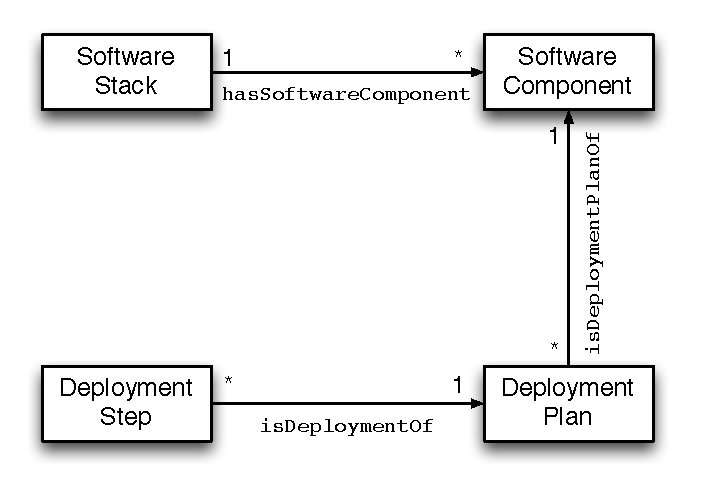
\includegraphics[width=0.9\linewidth]{figures/stack-rel}
	\caption{Overview of the WICUS software stack relation diagram.}
	\label{fig:stack-rel}
\end{figure}

Listing \ref{lst:plan-soykb} shows an example of the abstract plan for the SoyKB workflow. 
The first section of the plan (lines 1--26) describes the deployment of the workflow 
management system (\texttt{Pegasus}~\cite{Deelman-FGCS-2014}) and its related 
dependencies. Note that this section is common across all deployment plans for the workflows 
covered in this work. The remaining lines describe how the SoyKB software is deployed. 
The \texttt{SOFTWARE.TAR.GZ} stack, which is a dependency for all SoyKB wrappers, is 
the first component to be deployed (lines 27--29). Finally, the last section of the plan (lines 
30--45) describes how the four SoyKB wrappers are deployed. For each wrapper, two 
deployment steps are required: 1)~copy of the program execution binary, and 2)~the
 granting of proper execution permissions.}

\begin{lstlisting}[caption={Abstract deployment plan of the SoyKB WF.}, label={lst:plan-soykb}, basicstyle=\scriptsize]
OPEN_SSH_CLIENTS_SOFT_STACK stack
  OPEN_SSH_CLIENTS_SOFT_COMP component
    OPEN_SSH_CLIENTS_DEP_STEP step
OPEN_SSH_SERVER_SOFT_STACK stack
  OPEN_SSH_SERVER_SOFT_COMP component
    OPEN_SSH_SERVER_DEP_STEP step
WGET_SOFT_STACK stack
  WGET_SOFT_COMP component
    WGET_DEP_STEP step
CONDOR_CENTOS_6_5_SOFT_STACK stack
  CONDOR_CENTOS_6_5_SOFT_COMP component
    STOP_CONDOR_DEP_STEP step
    ADD_CONDOR_REPO_DEP_STEP step
    CONDOR_YUM_INSTALL_DEP_STEP step
    CLEAN_AND_SET_CONDOR_DEP_STEP step
    RESTART_DAEMONS_DEP_STEP step
JAVA-1.7.0-OPENJDK.X86_64_SOFT_STACK stack
  JAVA-1.7.0-OPENJDK.X86_64_SOFT_COMP component
    JAVA-1.7.0-OPENJDK.X86_64_DEP_STEP step
JAVA-1.7.0-OPENJDK-DEVEL.X86_64_SOFT_STACK stack
  JAVA-1.7.0-OPENJDK-DEVEL.X86_64_SOFT_COMP component
    JAVA-1.7.0-OPENJDK-DEVEL.X86_64_DEP_STEP step
PEGASUS_WMS_CENTOS_6_5_SOFT_STACK stack
  PEGASUS_WMS_CENTOS_6_5_SOFT_COMP component
    ADD_PEGASUS_REPO_DEP_STEP step
    PEGASUS_YUM_INSTALL_DEP_STEP step
SOFTWARE_TAR_GZ_SOFT_STACK stack
  SOFTWARE_TAR_GZ_SOFT_COMP component
    SOFTWARE_TAR_GZ_DEP_STEP step
PICARD-WRAPPER_SOFT_STACK stack
  PICARD-WRAPPER_SOFT_COMP component
    PICARD-WRAPPER_DEP_STEP step
    PICARD-WRAPPER_2_DEP_STEP step
SOFTWARE-WRAPPER_SOFT_STACK stack
  SOFTWARE-WRAPPER_SOFT_COMP component
    SOFTWARE-WRAPPER_DEP_STEP step
    SOFTWARE-WRAPPER_2_DEP_STEP step
GATK-WRAPPER_SOFT_STACK stack
  GATK-WRAPPER_SOFT_COMP component
    GATK-WRAPPER_DEP_STEP step
    GATK-WRAPPER_2_DEP_STEP step
BWA-WRAPPER_SOFT_STACK stack
  BWA-WRAPPER_SOFT_COMP component
    BWA-WRAPPER_DEP_STEP step
    BWA-WRAPPER_2_DEP_STEP step
\end{lstlisting}



